Soit $G$ un groupe et $E$ iun ensemble. On dit que $G$ agit sur $E$ s'il existe une application 
$\fonction \varphi {G \times E} E {(g,x) }{\varphi(g,x) = g \cdot x}$ telle que 
$\forall x \in E, e \cdot x = x$ et $\forall g,h \in G, \forall x \in E, g \cdot (h \cdot x) = (gh) \cdot x$.

\begin{remarque}
   $\forall g \in G$, $\fonction{\varphi_g}{E}{E}{x}{g \cdot x}$ est bijective, car son inverse est $\varphi_{g^{-1}}$.
\end{remarque}

De façon équivalente, se donner une action de groupe, c'est se donner un morphisme 
de groupes $\fonction{}{(G, \times)} {(\operatorname{Bij} E, \circ)}{g}{\varphi_g}$.

\section*{Exemples usuels}

\begin{enumerate}
    \item Si $G \subset S_n =$ groupe des permutations, alors $G$ agit sur $[1,n]$.
    \[
    \begin{aligned}
        G \times [1,n] &\to [1,n] \\
        (\sigma, i) &\mapsto \sigma(i)
    \end{aligned}
    \]

    \item Tout groupe $G$ agit sur lui-même par conjugaison :
    \[
    \begin{aligned}
        G \times G &\to G \\
        (g, x) &\mapsto gxg^{-1}
    \end{aligned}
    \]

    \item Tout groupe $G$ agit sur lui-même par translation :
    \[
    \begin{aligned}
        G \times G &\to G \\
        (g, x) &\mapsto gx
    \end{aligned}
    \]

    \item $\mathbb{K}$ un corps, $GL_n(\mathbb{K})$ agit sur $\mathbb{K}^n$
    \[
    \begin{aligned}
        GL_n(\mathbb{K}) \times \mathbb{K}^n &\to \mathbb{K}^n \\
        (M, x) &\mapsto Mx
    \end{aligned}
    \]
    agit aussi sur $Gr_k(\mathbb{K}^n) = \{ \text{sev de dim } k \text{ de } \mathbb{K}^n \}$ (grassmanienne).
    \[
    \begin{aligned}
        GL_n(\mathbb{K}) \times Gr_k(\mathbb{K}^n) &\to Gr_k(\mathbb{K}^n) \\
        (M, V) &\mapsto MV
    \end{aligned}
    \]
\end{enumerate}


\noindent \textbf{Exo :} $\mathbb{K} = \mathbb{Z}/p\mathbb{Z}$, $GL_n(\mathbb{Z}/p\mathbb{Z})$, cardinal ? \\
card sev de dim $k$ de $(\mathbb{Z}/p\mathbb{Z})^n$ ? \\
Dessiner droites vectorielles de $(\mathbb{Z}/3\mathbb{Z})^2$.

\vspace{0.5cm}

\section*{\underline{Vocabulaire lié aux actions de groupes}}

Soit $\fonction{}{G \times E} E {(g, x)} {g\cdot x}$ une action de $G$ sur $E$, et soit $x \in E$ fixé. \\


 $O(x) = \{ g \cdot x \mid g \in G \} \subset E$ (orbite)

\vspace{0.3cm}

\noindent \textbf{Affirmation :} l'ensemble des orbites forme une partition de $E$.
\begin{itemize}
    \item Si $x \in E$, $x \in O(x)$ car $x = e \cdot x$.
    \item Supposons que $O(x) \cap O(y) \neq \emptyset$. \\
    Alors $\exists g, g'$ tels que $gx = g'y$, donc $(g')^{-1}g \cdot x = y$. \\
    Donc $y \in O(x)$.
    \item Si $h \cdot y \in O(y)$, $h \cdot y = h \cdot ((g')^{-1}g \cdot x) = (h (g')^{-1} g) \cdot x \in O(x)$. \\
    Donc $O(x) = O(y)$.
\end{itemize}

\vspace{0.3cm}

\noindent \textbf{Cas particulier :} on dit que $G$ agit \textit{transitivement} sur $E$ si : \\
$\forall x, y \in E, \exists g, g x = y$. \\
$E$ est alors constitué d'une seule orbite.

\vspace{0.3cm}

$\to$ Relation d'équivalence sur $E$, on a $x \sim y \iff \exists g \in G, gx = y$ \\
\hspace*{6cm} $\iff O(x) = O(y)$.

\vspace{0.3cm}

\noindent \rule{\textwidth}{0.5pt}

Soit $x \in E$ : on note $G_x = \{ g \in G \mid g \cdot x = x \} \subset G$. 
$G_x$ est un sous-groupe de $G$, appelé \textit{stabilisateur} de $x$.

Soient $x, y \in E$, $g \in G$ tel que $g \cdot x = y$. \\
Donc $h \cdot y = y \iff h \in G_y$ \\
\hspace*{2.2cm} $\iff h \cdot (gx) = gx \iff (g^{-1}hg) \cdot x = x \iff g^{-1}hg \in G_x$ \\
\hspace*{2.2cm} $\iff h \in g G_x g^{-1}$.


$G_y = g G_x g^{-1}$ : $G_x$ et $G_y$ sont conjugués, et en particulier si $G$ est fini,
\[
O(x) = O(y) \implies |G_x| = |G_y|.
\]

\vspace{0.5cm}

\begin{theoreme}{}{}  
    Soit $G$ agissant sur $E$, et $x \in E$. Alors
\[
\begin{aligned}
    G/G_x &\xrightarrow{(*)} O(x) \\
    gG_x &\longmapsto g \cdot x
\end{aligned}
\]
est bien définie et bijective.

\end{theoreme}
{\footnotesize (Note : $G/G_x = \{ gG_x, g \in G \}$ ensemble des classes à gauche modulo $G_x$).}

\vspace{0.3cm}

\begin{proof}
    
\begin{align*}
    g_1 G_x = g_2 G_x &\iff g_2^{-1} g_1 G_x = G_x \\
    &\iff g_2^{-1} g_1 \in G_x \\
    &\iff g_2^{-1} g_1 \cdot x = x \\
    &\iff g_1 x = g_2 x
\end{align*}
$\implies$ déf de $(*)$ \\
$\Longleftarrow$ $(*)$ est injective.

\noindent Surjectivité évidente.

\end{proof}

\vspace{0.5cm}

\begin{corollaire}{}{} Si $G$ est fini, $\forall x \in E$, $|G| = |G_x| \times |O(x)|$.
\end{corollaire}
\vspace{0.5cm}

\noindent \uline{Repris exo précédent :} $(GL_n(\mathbb{Z}/p\mathbb{Z}), \times)$ est un groupe fini. \\
$\to$ combien de matrices inversibles à coeffs dans $\mathbb{Z}/p\mathbb{Z}$ ?

Inversible :
\[
\begin{bmatrix}
    \vert & \vert & & \vert \\
    C_1 & C_2 & \dots & C_n \\
    \vert & \vert & & \vert
\end{bmatrix}
\implies C_1, C_2, \dots, C_n \text{ base de } \mathbb{K}^n.
\]

Soit $C_1 \in \mathbb{K}^n \setminus \{0\}$, alors $p^n - 1$ choix. \\
$C_2 \notin \underbrace{\text{Vect}(C_1)}_{\text{cardinal} p} = \{ \lambda C_1 \mid \lambda \in \mathbb{Z}/p\mathbb{Z} \}$ \\

Donc choix possibles pour $C_2 : p^n - p$. \\
Choix pour $C_3 : \mathbb{K}^n \setminus \text{Vect}(C_1, C_2) \implies p^n - p^2$ choix.

et donc $C_n \in \mathbb{K}^n \setminus \text{Vect}(C_1, \dots, C_{n-1})$ : $p^n - p^{n-1}$ choix.

\vspace{0.5cm}

\begin{theoreme}{}{}
\begin{align}
    |GL_n(\mathbb{Z}/p\mathbb{Z})| & = \prod_{i=0}^{n-1} (p^n - p^i) \\
    & = (p^n - 1)(p^n - p)(p^n - p^2) \dots (p^n - p^{n-1}) \\
    & = p^{n - 1}(p - 1) p^{n - 2}(p^2 - 1) \dots p^1 (p^{n-1} - 1) p^0 (p^n - 1) \\
    & = p^{\frac{n(n - 1)}{2}} \prod_{k=1}^n (p^k - 1)
\end{align}
\end{theoreme}

\vspace{0.8cm}


Soit $E$ un ev de dim finie et $V, W$ deux sev de dim $k$. Alors $\exists \phi \in GL(E)$ tel que $\phi(V) = W$. \\
Donc l'action suivante est \textit{transitive}.
\[
\begin{aligned}
    GL_n \times Gr_k &\to Gr_k \\
    (M, V) &\mapsto M(V)
\end{aligned}
\]

\vspace{0.3cm}

$V = \text{Vect}(e_1, \dots, e_k)$, alors $O(V) = Gr_k$ donc $G_n / G_V \to Gr_k$ bijective, avec $G_V$ stabilisateur. \\
et $|Gr_k| \times |G_V| = |G_n|$ 

\vspace{0.3cm}

$$M \in G_V \iff M = \left[ \begin{array}{c|c}
    A & B \\
    \hline
    0 & D
\end{array} \right] $$

Avec $A$ et $D$ inversibles de taille $k$ et $n-k$, et B matrice quelconque de taille $k \times (n-k)$. Il y a donc 
$p{k(n-k)}$ choix pour $B$.

Pour que $M$ soit inversible, il faut les diagonales inversibles.

Donc $G/G_V \to Gr_k$ est bijective.

\vspace{0.8cm}

\underline{$k=1$ :} nombre de droites vectorielles de $(\mathbb{Z}/p\mathbb{Z})^n$.

\noindent \textbf{Aff :} il y en a $\frac{p^n - 1}{p-1}$.

\vspace{0.5cm}

$n=2, p=3 \implies 4$ droites vectorielles.



\begin{center}
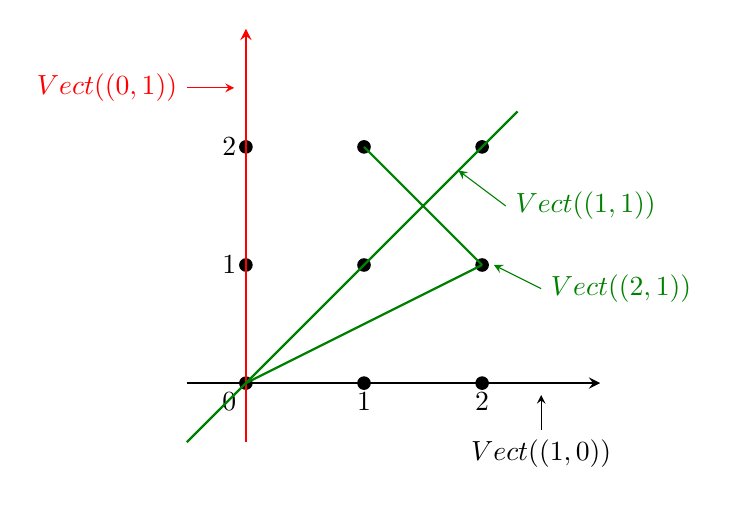
\begin{tikzpicture}[scale=1.5, >=stealth]
    % Grille des points (Z/3Z)^2
    \foreach \x in {0,1,2}
        \foreach \y in {0,1,2}
            \filldraw (\x,\y) circle (1.5pt);

    % Étiquettes des axes
    \node[below left] at (0,0) {0};
    \node[below] at (1,0) {1};
    \node[below] at (2,0) {2};
    \node[left] at (0,1) {1};
    \node[left] at (0,2) {2};

    % 1. Droite Vect((1,0)) - Axe horizontal
    \draw[->, thick] (-0.5, 0) -- (3, 0);
    \draw[<-] (2.5, -0.1) -- (2.5, -0.4) node[below] {$\text{Vect}((1,0))$};

    % 2. Droite Vect((0,1)) - Axe vertical (Rouge)
    \draw[->, thick, red] (0, -0.5) -- (0, 3);
    \draw[<-, red] (-0.1, 2.5) -- (-0.5, 2.5) node[left] {$\text{Vect}((0,1))$};

    % 3. Droite Vect((1,1)) - Diagonale
    \draw[thick, green!50!black] (-0.5, -0.5) -- (2.3, 2.3);
    \draw[<-, green!50!black] (1.8, 1.8) -- (2.2, 1.5) node[right] {$\text{Vect}((1,1))$};

    % 4. Droite Vect((2,1))
    % Segment de l'origine à (2,1)
    \draw[thick, green!50!black] (0, 0) -- (2, 1);
    % Segment demandé reliant (1,2) à (2,1)
    \draw[thick, green!50!black] (1, 2) -- (2, 1);
    
    % Annotation
    \draw[<-, green!50!black] (2.1, 1) -- (2.5, 0.8) node[right] {$\text{Vect}((2,1))$};

\end{tikzpicture}
\end{center}